\section{From waveform to feature window}
The preprocessing is deliberately plain, because it has to behave identically in three places: when features are cached for training, when Part~2 scores a test file, and when a user uploads a recording to the application. The steps are:
\begin{enumerate}
  \item Load the WAV file with \texttt{soundfile} as 32-bit floating point, keeping both channels.
  \item Resample a channel only if its rate differs from 16\,kHz. In practice this branch never ran, since every audited file is already at 16\,kHz.
  \item Compute, for each channel, a Mel power spectrogram with \texttt{librosa} \cite{librosa}, using an FFT length of 1024 samples (64\,ms), a hop of 512 samples (50\,\%), 128 Mel bands and power~2, and convert it to decibels with the same formula as the official baseline,
  \begin{equation}
    X_{t,m} = \frac{20}{p}\,\log_{10}\!\big(\max(S_{t,m},\varepsilon)\big), \qquad p = 2,\quad \varepsilon = 2.2\times 10^{-16},
    \label{eq:logmel}
  \end{equation}
  where $S_{t,m}$ is the Mel power in frame $t$ and band $m$.
  \item Concatenate the two 128-band frames of the same time step into one 256-dimensional frame, and replace any non-finite value.
  \item Standardise each of the 256 dimensions with the mean $\mu_m$ and standard deviation $\sigma_m$ computed over the training frames of the model in use: $\tilde X_{t,m} = (X_{t,m}-\mu_m)/\sigma_m$. These statistics are stored in the checkpoint, so inference never needs the training data.
  \item Form overlapping windows of five consecutive frames (stride one) and flatten each to a 1280-dimensional vector.
\end{enumerate}
A 10\,s clip gives 309 windows, an 11\,s clip 340 and a 12\,s clip 372. We neither pad nor crop clips of different lengths; the model sees windows, so a longer clip simply contributes more of them. Features of all training recordings are extracted once per machine and cached, which made the fourteen training runs considerably faster than re-reading the audio each epoch would have been.

\section{Why both channels, and why standardise}
We kept both channels because the difference between the two domains in this task lies in the acoustic conditions, and whatever the second channel adds about the surrounding noise is exactly the information a noise-aware detector should see. Concatenating the two channels was the least intrusive way to use them: the Autoencoder needs a wider first and last layer and nothing else changes.

Standardisation is the other departure from the baseline. Raw log-Mel values span tens of decibels and differ systematically between low and high bands, so without standardisation the reconstruction loss is dominated by the loudest bands and by the overall decibel offset. An early single-machine prototype that trained on unnormalised features produced losses in the hundreds that said little about how well the model was doing. With per-dimension z-scoring every band carries comparable weight and the losses, shown in Figure~\ref{fig:losses}, are of order one.

\begin{figure}[!htb]\centering
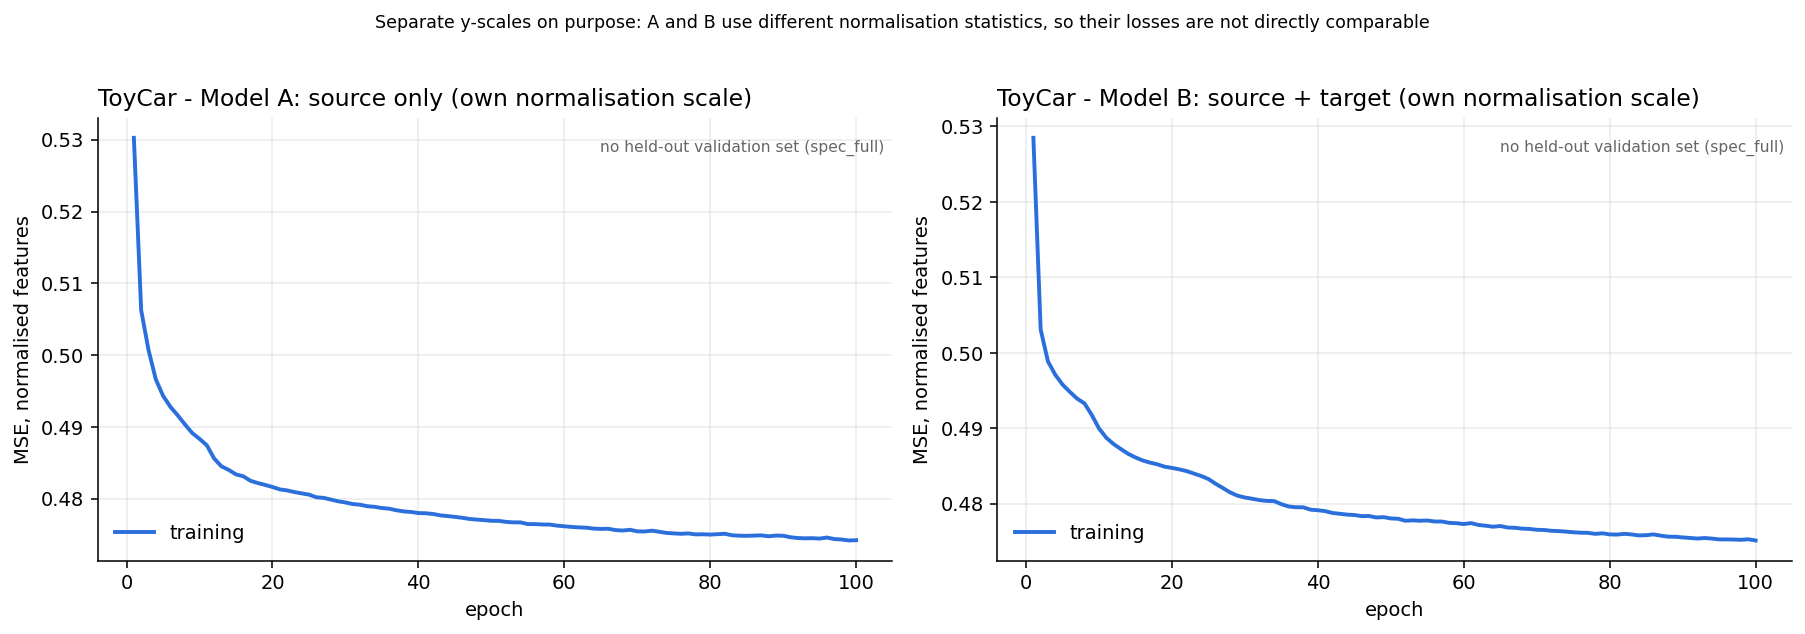
\includegraphics[width=0.9\textwidth]{ToyCar_training_curves_per_model}
\caption{Training loss of the two ToyCar models, Model~A on the left and Model~B on the right. Each panel is on its own normalisation scale. The annotation records that no held-out validation set exists under the adopted protocol.}
\label{fig:toycarloss}
\end{figure}
